\chapter{I/O Connectors and Jumpers}

\section*{Connectors}

The \jr\ has several connectors on its board for I/O devices beyond the standard connections on the back. Some of these connectors are the only way to access that particular I/O device, but some are auxiliary connectors that provide alternate forms of access. All are IDC header pins. The diagrams that follow show the pin assignments for these connectors. In these diagrams, the views are top-down onto the board, with the board arranged so that the main connectors are towards the top and the power connector is towards the bottom.

\subsection*{Game Connectors}

There are two connectors for game controllers. There are two connectors for Atari style joysticks (figure~\ref{fig:port_joy}). And two for NES or Super NES gamepads (figure~\ref{fig:port_nes}).

For the Atari style joysticks, an adapter cable will be needed to convert from IDC to the standard DB-9 connector. There are two key differences between the \jr\ and Atari or Commodore devices: first, the \jr\ provides 3.3 volts instead of 5 volts, and second there are no paddle inputs supported on the \jr.

For the NES and SNES style gamepads, an adapter box will be needed to provide the correct interfacing for a controller. This adapter should be available from Foenix Retro Systems in the near future (at the time of writing this manual).

\begin{figure}[ht]
    \begin{center}
        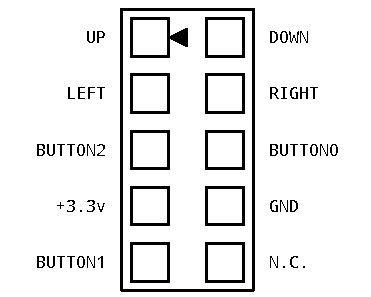
\includegraphics[scale=0.75]{images/f256_port_joystick.pdf}
    \end{center}
    \caption{Joystick Port Pinouts}
    \label{fig:port_joy}
\end{figure}

\begin{figure}[ht]
    \begin{center}
        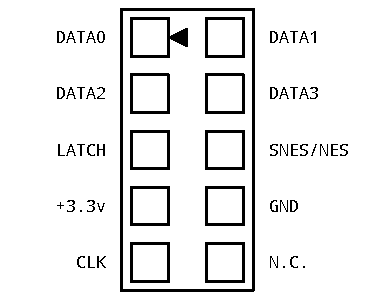
\includegraphics[scale=0.75]{images/f256_port_nes.pdf}
    \end{center}
    \caption{NES/SNES Gamepad Port Pinouts}
    \label{fig:port_nes}
\end{figure}

\subsection*{PS/2 Port}

An internal connector is included for the PS/2 mouse and keyboard port (figure~\ref{fig:port_ps2}). This connector just provides an alternate way of accessing the PS/2 signals. It could be useful in building an integrated case for the \jr\ that includes a PS/2 keyboard.

\begin{figure}[ht]
    \begin{center}
        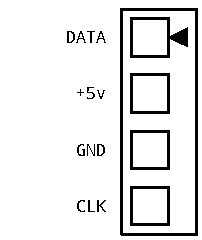
\includegraphics[scale=0.75]{images/f256_port_ps2.pdf}
    \end{center}
    \caption{Auxiliary PS/2 Pinouts}
    \label{fig:port_ps2}
\end{figure}

\subsection*{UART}

This connector provides access to the serial in and out signals for the \jr's UART (figure~\ref{fig:port_uart}). The TxD and RxD signals are compatible with standard $\pm 12$ volt RS-232 signals. The signals on this connector can be brought out to a DB-9 connector to provide a standard 3 wire RS-232 serial port.

\begin{figure}[ht]
    \begin{center}
        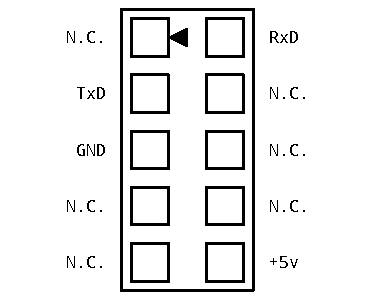
\includegraphics[scale=0.75]{images/f256_port_uart.pdf}
    \end{center}
    \caption{UART Pinouts}
    \label{fig:port_uart}
\end{figure}

NOTE: a ESP32 Feather board can be installed on the \jr\ to provide access to Wi-Fi, but using this board will take over the supplied UART. Therefore, the \jr\ can provide either an RS-232 serial port or access to Wi-Fi, but not both at the same time. A jumper on the board selects which is active.

\subsection*{USB Debug Port}

While there is a USB Mini-B connector (figure:~\ref{fig:port_usb}) on the port to access the USB debug interface, there is an IDC header connector on the board to provide access to this for the case USB connector, if desired. This is not compatible with all USB case connectors, as many of them are dual connectors and require pins for two USB ports. It should be compatible with cases with single connectors or with panel mounted USB cables.

\begin{figure}[ht]
    \begin{center}
        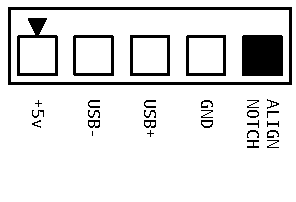
\includegraphics[scale=0.75]{images/f256_port_usb.pdf}
    \end{center}
    \caption{USB Debug Pinouts}
    \label{fig:port_usb}
\end{figure}

\subsection*{Case Connectors}

There are two connectors for the usual PC case connections. There is one for the headphone jack (figure:~\ref{fig:port_audio}), and one for the various buttons, LEDs, and case speaker (figure:~\ref{fig:port_case}): power, reset, hard drive/SD card activity. Note that while the speaker and buttons are not polarized, the power LED and hard-drive activity LED are and must be wired in the correct orientation.

\begin{figure}[ht]
    \begin{center}
        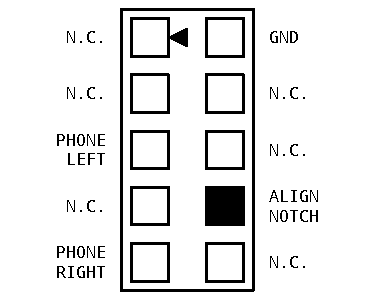
\includegraphics[scale=0.75]{images/f256_port_audio.pdf}
    \end{center}
    \caption{Case Audio Pinouts}
    \label{fig:port_audio}
\end{figure}

\begin{figure}[ht]
    \begin{center}
        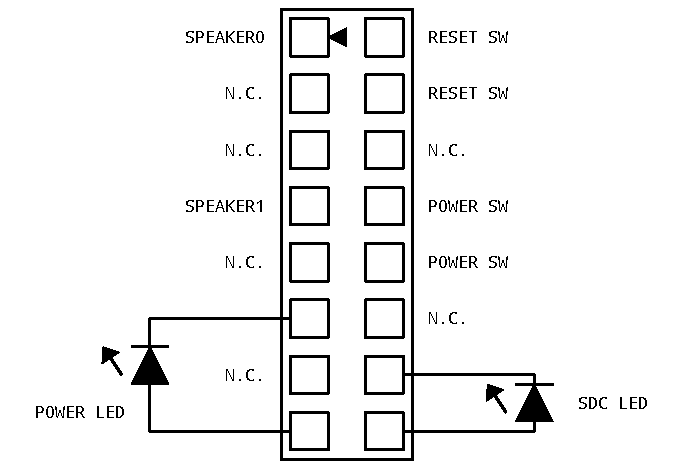
\includegraphics[scale=0.75]{images/f256_port_case.pdf}
    \end{center}
    \caption{Case Button and LED Pinouts}
    \label{fig:port_case}
\end{figure}

NOTE: not shown is a small secondary connector for an SPST switch for power (the connector is located at the front-right corner of the \jr\ RevB board). This connector provides an alternative to the usual case power push button. The two buttons cannot be used together. Either the case push button shown in \ref{fig:port_case} is used, or the other SPST switch is used, but not both.

\section*{Jumpers}

There are several IDC header pins with jumpers to configure various options on the \jr. All the jumper headers are three pin headers, where the center pin is the common. The header is used to select the appropriate routing of a signal or voltage level. So the jumper is always used to connect the center common pin to either the left or right pins (or the top or bottom, depending on the orientation of the header).

\subsection*{SID Jumpers}

The SID chips have two sets of jumpers each. The first pair are the voltage selection jumpers. They can be used to select the appropriate voltage for the SID chip: 12 volts for the original 6581, and 9 volts for the later 8580 (see figure~\ref{fig:jmp_sid_voltage}). If you are using a modern replacement, check the instructions as to which voltage to use: some replacements work with either voltage.

\begin{figure}[ht]
    \begin{center}
        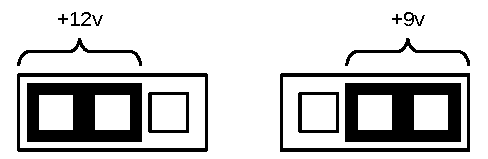
\includegraphics[scale=0.75]{images/jumper_voltage.pdf}
    \end{center}
    \caption{SID Voltage Jumper}
    \label{fig:jmp_sid_voltage}
\end{figure}

The second pair of SID jumpers are the channel selectors (see figure~\ref{fig:jmp_sid_channel}). These jumpers select the source of the left and right channels for the CODEC. With each one, you can select either the right or the left SID as an input to the CODEC for that stereo channel. If a \jr\ is using both SIDs, the left channel should select the left SID, and the right channel select the right SID. But if only a single SID is used, both channels can be set to that SID. For instance, if the SID is in the left socket, both left and right channels can select the left SID as the source to get a balanced monaural sound.

\begin{figure}[ht]
    \begin{center}
        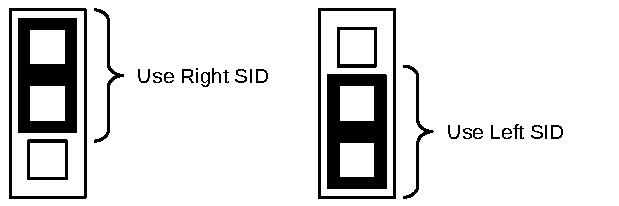
\includegraphics[scale=0.75]{images/jumper_channel.pdf}
    \end{center}
    \caption{SID Stereo Channel Source Jumper}
    \label{fig:jmp_sid_channel}
\end{figure}

\subsection*{Boot Source}

For the \jr\ RevB, there is a jumper to select boot source (see figure~\ref{fig:jmp_boot}). With the jumper in the left position, the \jr\ will boot off the flash, using the last 8KB bank of flash memory as the last 8KB of CPU address space. With the jumper in the right position, the \jr\ will boot using RAM. On the RevA boards, this jumper is not present, and so this feature is controlled by a command on the USB debug port, which the RevB board does not support. See page~\ref{pg:mmu_boot_config} for a more complete description of boot sources.

\begin{figure}[ht]
    \begin{center}
        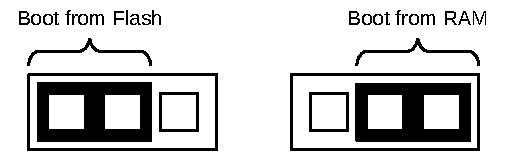
\includegraphics[scale=0.75]{images/jumper_boot.pdf}
    \end{center}
    \caption{Boot Source Jumper}
    \label{fig:jmp_boot}
\end{figure}

\subsection*{UART Configuration}

There are two headers for selecting how the UART is used---selecting between the serial port or the ESP32 Wi-Fi module (see figure~\ref{fig:jmp_uart}). One jumper controls the routing of the TxD line, while the other controls the routing of the RxD line. With the jumper positioned across the ``back'' pair of pins, the signal is routed to the Wi-Fi module. With the jumper positioned across the ``front'' pair of pins, the signal is routed to the DB-9 port connected to the UART connector. Note that both the TxD and RxD jumpers should be in the same relative position so that they both use the same device.

\begin{figure}[ht]
    \begin{center}
        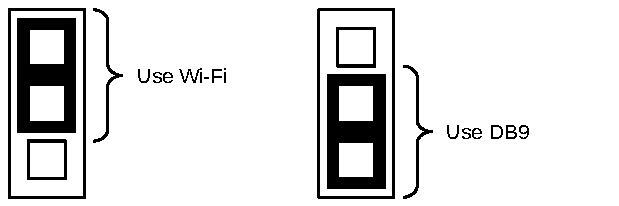
\includegraphics[scale=0.75]{images/jumper_uart.pdf}
    \end{center}
    \caption{UART Device Jumpers}
    \label{fig:jmp_uart}
\end{figure}